\section{Beispiel: Gleichverteilung}
\index{Gleichverteilung}
Als Beispiel und zur Gegenüberstellung stetiger und diskreter Zufallsvariablen
behandeln wir in diesem Abschnitt die diskrete und die stetige
Gleichverteilung.
Weitere Informationen zur Gleichverteilung sind
im Abschnitt~\ref{section-gleichverteilung-stetig} zu finden.

\subsection{Ganzzahlige Gleichverteilung}
\index{Gleichverteilung!ganzzahlig}
Eine Zufallsvariable $X$ nehme die ganzzahligen Werte $\{a,a+1,\dots,b\}$ mit 
gleicher Wahrscheinlichkeit $\frac1{b-a+1}$ an.
Die Verteilungsfunktion
(Abbildung~\ref{diskrete-gleichverteilung})
ist also
\[
F(x)=
\frac{\lfloor x \rfloor -a+1}{b-a+1}
\]
wobei $\lfloor x \rfloor$ die grösste ganze Zahl kleiner als $x$
bezeichnet:
\[
\lfloor x\rfloor = \max\{k\in\mathbb Z|k\le x\}.
\]
Die Wahrscheinlichkeitsverteilung ist
\[
P(X=x)=\begin{cases}
\displaystyle \frac1{b-a+1}&\qquad a\le x\le b,x\in\mathbb Z\\
0&\qquad\text{sonst}.
\end{cases}
\]
Damit kann jetzt auch Erwartungswert und Varianz bestimmt werden.
{\allowdisplaybreaks
\begin{align*}
E(X)
&=
\sum_{k=a}^b kP(X=k)
=
\sum_{k=a}^b \frac{k}{b-a+1}
=
\frac1{b-a+1}\sum_{k=a}^bk
\\
&=
\frac1{b-a+1}\biggl(
\sum_{k=1}^bk-\sum_{k=1}^{a-1}k
\biggr)
=
\frac1{b-a+1}\biggl(
\frac{b(b+1)}2-\frac{a(a-1)}2
\biggr)
\\
&=
\frac12\frac{b^2+b-a^2+a}{b-a+1}=\frac{a+b}2,
\\
E(X^2)
&=
\sum_{k=a}^b k^2P(X=k)
=
\sum_{k=a}^b \frac{k^2}{b-a+1}
=
\frac1{b-a+1}\sum_{k=a}^bk^2
\\
&=
\frac1{b-a+1}\biggl(
\sum_{k=1}^bk^2-\sum_{k=1}^{a-1}k^2
\biggr)
=
\frac{ 2(a^2+ab+b^2)+b-a}{6},
\\
\operatorname{var}(X)
&=
\frac{ 2(a^2+ab+b^2)+b-a}{6}
-
\frac{a^2+2ab+b^2}{4}
\\
&=
\frac1{12}\bigl(
4a^2+4ab+4b^2+2b-2a-3a^2-6ab-3b^2
\bigr)
\\
&=
\frac1{12}\bigl(
a^2-2ab+b^2+2b-2a+1-1
\bigr)
=
\frac1{12}\bigl((b-a+1)^2 - 1\bigr).
\end{align*}
}
Die Varianz ist also im Wesentlichen die quadrierte Intervalllänge
geteilt durch 12.
\begin{figure}
\centering
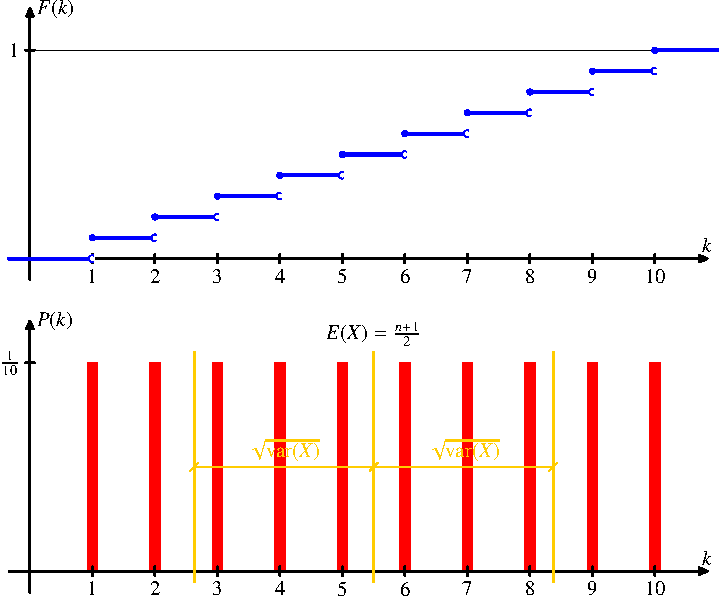
\includegraphics{images/gl-2.pdf}
\caption{Verteilungsfunktion und Wahrscheinlichkeitsverteilung der diskreten
Gleichverteilung auf den Werten $1,\dots,n=10$
\label{diskrete-gleichverteilung}}
\end{figure}

\subsection{Stetige Gleichverteilung}
\begin{figure}
\centering
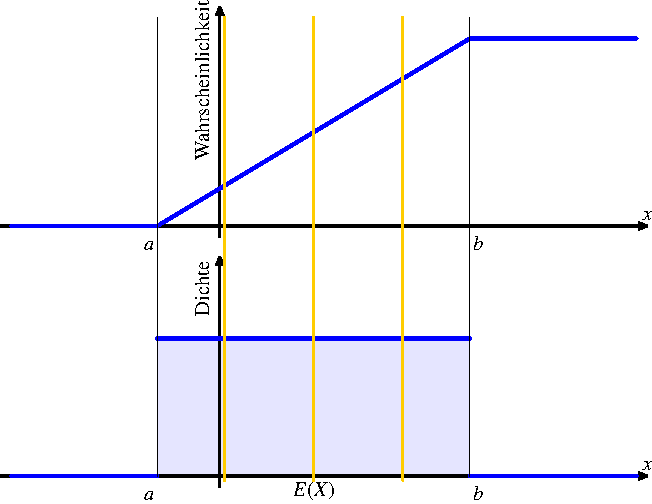
\includegraphics{images/verteilungsfunktion-7.pdf}
\caption{Verteilungsfunktion und Wahrscheinlichkeitsdichte der stetigen
Gleichverteilung im Intervall $[a,b]$
\label{stetige-gleichverteilung}}
\end{figure}
\index{Gleichverteilung!stetig}
\index{Gleichverteilung!auf einem Intervall}
Eine Zufallsvariable $X$ nehme die Werte im Intervall $[a,b]$
mit gleicher Wahrscheinlichkeit an, d.~h.~für jedes Teilintervall
$[\xi,\eta]\subset[a,b]$ gilt 
\[
P(\xi\le X\le \eta)=\frac{\xi-\eta}{b-a}.
\]
Die Wahrscheinlichkeitsdichte ist dann (Abbildung~\ref{stetige-gleichverteilung})
\[
\varphi(x)=\begin{cases}
\displaystyle \frac1{b-a}&\qquad a\le x\le b\\
0&\qquad \text{sonst}
\end{cases}
\]
Erwartungswert und Varianz können damit direkt berechnet werden:
{\allowdisplaybreaks
\begin{align*}
E(X)
&=
\int_{-\infty}^\infty x\varphi(x)\,dx
=
\int_a^bx\frac1{b-a}\,dx
=
\frac1{b-a}\left[\frac12x^2\right]_a^b
=
\frac12\frac{b^2-a^2}{b-a}
\\
&=
\frac{a+b}2,
\\
E(X^2)
&=
\int_{-\infty}^{\infty}x^2\varphi(x)\,dx
=
\int_a^bx^2\frac1{b-a}\,dx
=
\frac1{b-a}\left[\frac13x^3\right]_a^b
=
\frac13\frac{b^3-a^3}{b-a}
\\
&=
\frac13(b^2+ab+a^2),
\\
\operatorname{var}(X)
&=
\frac13(b^2+ab+a^2)
-
\frac14(a^2+2ab+b^2)
\\
&=
\frac1{12}(4b^2+4ab+4a^2-3a^2-6ab-3b^2
=
\frac1{12}(a^2-2ab+b^2)
\\
&=
\frac{(b-a)^2}{12}.
\end{align*}
}
Auch in diesem Fall ist die Varianz die quadrierte Intervalllänge
geteilt durch 12.

